\documentclass[a4paper,10pt]{article}
\usepackage{listings}
\usepackage{color}
\usepackage{algorithm2e}
\usepackage{graphicx}
\usepackage{epstopdf}
\usepackage[margin=1.0in]{geometry}
\usepackage{amsmath,amsthm,amssymb}
 
\definecolor{dkgreen}{rgb}{0,0.6,0}
\definecolor{gray}{rgb}{0.5,0.5,0.5}
\definecolor{mauve}{rgb}{0.58,0,0.82}
 
\lstset{ %
  language=C++,                % the language of the code
  basicstyle=\footnotesize,           % the size of the fonts that are used for the code
  numbers=left,                   % where to put the line-numbers
  numberstyle=\tiny\color{gray},  % the style that is used for the line-numbers
  stepnumber=1,                   % the step between two line-numbers. If it's 1, each line 
                                  % will be numbered
  numbersep=5pt,                  % how far the line-numbers are from the code
  backgroundcolor=\color{white},      % choose the background color. You must add \usepackage{color}
  showspaces=false,               % show spaces adding particular underscores
  showstringspaces=false,         % underline spaces within strings
  showtabs=false,                 % show tabs within strings adding particular underscores
  frame=single,                   % adds a frame around the code
  rulecolor=\color{black},        % if not set, the frame-color may be changed on line-breaks within not-black text (e.g. commens (green here))
  tabsize=2,                      % sets default tabsize to 2 spaces
  captionpos=b,                   % sets the caption-position to bottom
  breaklines=true,                % sets automatic line breaking
  breakatwhitespace=false,        % sets if automatic breaks should only happen at whitespace
  title=\lstname,                   % show the filename of files included with \lstinputlisting;
                                  % also try caption instead of title
  keywordstyle=\color{blue},          % keyword style
  commentstyle=\color{dkgreen},       % comment style
  stringstyle=\color{mauve},         % string literal style
  escapeinside={\%*}{*)},            % if you want to add LaTeX within your code
  morekeywords={*,...}               % if you want to add more keywords to the set
}

% Title Page
\title{Assignment 1: Introduction to Systems Programming}
\author{Kevin Rich, Francis Vo, Soo-Hyun Yoo}

\setlength{\parindent}{0cm}
\setlength{\parskip}{1em}


\begin{document}
	\maketitle

	\section{Mathematical Analysis}
		\subsection{Algorithm 1}
			\begin{algorithm}[H]
				\SetAlgoLined
				\LinesNumbered
				\DontPrintSemicolon
				\KwData{Integer array A of size N}
				\KwResult{Greatest Sum of Subarray}
				\For{$i \gets 0$ \KwTo $N$}{
					\For{$j \gets i$ \KwTo $N$}{
						$s \gets 0$\;
						\For{$k \gets i$ \KwTo $j$}{
							$s \gets s + A[k]$\;
						}
						\If{$s > max$}{
							 $max \gets s$\;
						}
					}
				}
			\caption{Pseudocode for Basic Enumeration}
			\end{algorithm}
			This Algorithm has 3 for-loops so it is O($n^3$).

		\subsection{Algorithm 2}
			\begin{algorithm}[H]
				\SetAlgoLined
				\LinesNumbered
				\DontPrintSemicolon
				\KwData{Integer array A of size N}
				\KwResult{Greatest Sum of Subarray}
				\For{$i \gets 0$ \KwTo $N$}{
					$s \gets 0$\;
					\For{$j \gets i$ \KwTo $N$}{
						 $s \gets A[j]$\;
						 \If{$s > max$}{
							 $max \gets s$\;
						 }
					}
				}
			\caption{Pseudocode for Better Enumeration}
			\end{algorithm}
			This Algorithm has 2 for-loops so it is O($n^2$).

		\subsection{Algorithm 3}
			\noindent {\bf Data}: Integer array A of size N \\
			{\bf Result}: Greatest Sum of Subarray

			\begin{minipage}[!h]{6in}
			\begin{verbatim}

			def MaxSubarray:
			    sums = MaxSubarray_recursive(A)
			    return max(sums)
			\end{verbatim}
			\end{minipage}

			\begin{center}
			\noindent {\bf Algorithm 3.1}: Starting function pseudocode for Divide and Conquer
			\end{center}

			\vspace{1em}
			
			\noindent {\bf Data}: Integer array A of size N \\
			{\bf Result}: Integer array of size 4

			\begin{minipage}[!h]{6in}
			\begin{verbatim}

			def MaxSubarray_recursive:
			    if A.size <= 1:
			        sums.all = A[0]
			        sums.left = A[0]
			        sums.right = A[0]
			        sums.overall = A[0]
			        return sums

			    left_sums = MaxSubarray_recursive(A, left_branch)
			    right_sums = MaxSubarray_recursive(A, right_branch)

			    sums.all = left_sums.all + right_sums.all
			    sums.left = max(left_sums.left, left_sums.all + right_sums.left)
			    sums.right = max(right_sums.right, left_sums.right + right_sums.all)
			    m = left_sums.right + right_sums.left
			    sums.overall = max(sums.all, sums.left, sums.right, m)

			    return sums
			\end{verbatim}
			\end{minipage}

			\begin{center}
			\noindent {\bf Algorithm 3.2}: Recursive function pseudocode for Divide and Conquer
			\end{center}

			\vspace{1em}

			\noindent This algorithm is recursive and decreases by half every step. Each lower step has double the number of calls. Thus, this algorithm is O($n \log n$).


	\newpage
	\section{Theoretical Correctness}

		{\bf Claim 1}: Given an array $a$ containing $n$ integers $a_0, a_1, \dots, a_{n-1}$ for $n > 0$, the divide-and-conquer algorithm (algorithm 3) correctly calculates the sum of the maximum subarray, $\displaystyle s = \max_{i\leq{j}} \left(\sum_{k=i}^j a_k\right),$ for integers $i,j<n$.

		We propose two methods of inductive proof: top-down and bottom-up.

  		The sum of all the elements in array denoted as sums.all\\
  		The largest sum starting from the left denoted as sums.left\\
  		The largest sum starting from the right denoted as sums.right\\
  		The overall max sum denoted as sums.overall\\
 
		{\bf Proof (top-down)}: As a base case, let $n=1$. Then sums.all = A[0], sums.left = A[0], sums.right = A[0], sums.overall = A[0]\\
  
  		For the inductive hypothesis, consider:\\
  			left\_sums = MaxSubarray\_recursive(A[0:$n \over 2$-1])\\
  			right\_sums = MaxSubarray\_recursive(A[$n \over 2$:n])\\
  			sums.all = left\_sums.all + right\_sums.all\\
  			sums.left = max(left\_sums.left, left\_sums.all + right\_sums.left)\\
  			sums.right = max(right\_sums.right, left\_sums.right + right\_sums.all)
  			sums.overall = max(sums.all, sums.left, sums.right, left\_sums.right + right\_sums.left)
  
		We can consider three cases:\\

  		{\it Case 1}: Contained entirely in the first half\\
  				This will be returned as left\_sums.overall from the recursive call on left\_sums.
  
  		{\it Case 2}: Contained entirely in the second half\\
  				This will be returned from the recursive call on right\_sums.
  
  		{\it Case 3}: Made of a suffix of the first half of maximun sum and the prefix of the second half of the maximum
  				This will be found using left\_sums.right + right\_sums.left

		\begin{center}
		$\Box$
		\end{center}

		{\bf Proof (bottom-up)}: As a base case, consider when $n=1$. Then {\tt MaxSubarray\_recursive($n$)} = $a_0$, which is true.

		For the inductive hypothesis, assume that for $n > 1$ and $n \leq q$ for some integer $q>1$, the algorithm correctly computes the sum of the maximum subarray.

		Consider an array of size $n=q+1$. Then we can consider one of four cases regarding the location of the maximum subarray within the whole array.

		{\it Case 1}: $\displaystyle s = a$. We correctly capture $s$ in {\tt sums.all}.

		{\it Case 2}: $\displaystyle s = \sum_{k=0}^j a_k$, for $j < q$. We correctly capture $s$ in {\tt sums.left}.

		{\it Case 3}: $\displaystyle s = \sum_{k=i}^q a_k$, for $i > 0$. We correctly capture $s$ in {\tt sums.right}.

		{\it Case 4}: $\displaystyle s = \sum_{k=i}^j a_k$, for $0 < i \leq j < q$. We correctly capture $s$ in {\tt m}.

		In all four cases, we correctly select the maximum sum among {\tt sums.all}, {\tt sums.left}, {\tt sums.right}, and {\tt m} as the sum of the maximum subarray of $a$.

		\begin{center}
		$\Box$
		\end{center}

		
		{\bf Claim 2}: The algorithm terminates.

		{\bf Proof}: Since $n>0$ per the problem statement, $n$ must be at least $1$, and the algorithm returns. This proves the base case.

		For the inductive hypothesis, assume that the algorithm returns for an array of length $n \leq q$ for some positive integer $q>1$. Consider $n=q+1$. The array will be split up into two branches of positive lengths, which means the branches will have lengths less than or equal to $q$. Thus, the algorithm will return for each branch, and the algorithm returns right afterwards.

		\begin{center}
		$\Box$
		\end{center}


		{\bf Claim 3}: The divide-and-conquer algorithm computes the sum of the maximum subarray in O($n \log n$) time.

		{\bf Proof}: Let $n$ be the size of the array of integers, $a$. For $n>1$, the recurrence for the recursive step of the algorithm can be found to be

		\begin{align*}
		T(n) &= \Theta(1) + 2T\left(\frac{n}{2}\right) + \Theta(n) + \Theta(1) \\
		     &= 2T\left(\frac{n}{2}\right) + \Theta(n),
		\end{align*}

		where

		\begin{itemize}
		\item The base case takes $\Theta(1)$,
		\item The recursive calls take $2T\left(\frac{n}{2}\right)$,
		\item The {\tt max()} calculations take $\Theta(n)$, and
		\item The final {\tt return} takes $\Theta(1)$.
		\end{itemize}

		In its entirety, \[T(n) = \begin{cases} \Theta(1) &\mbox{if } n = 1 \\ 2T\left(\frac{n}{2}\right) + \Theta(n) &\mbox{if } n > 1 \end{cases}.\]

		Suppose $T(n) \leq cn \log n + n = \text{O}(n \log n)$. Then

% 		As a base case, let $n=1$. Then $T(1) = c \log 1 + 1= \Theta(1)$, as desired.

% 		For the inductive hypothesis, assume $T(m) \leq cm \log m + m$ for $m < n$. Then if $m = \frac{n}{2}$,
		\begin{align*}
		T(n) &\leq 2\left(c \cdot \frac{n}{2} \log \frac{n}{2}\right) + n \\
		     &\leq cn \log \frac{n}{2} + n \\
		     &= cn \log n - cn \log 2 + n \\
		     &\leq cn \log n \\
		     &= \text{O}(n \log n),
		\end{align*}

		as desired.

		\begin{center}
		$\Box$
		\end{center}


	\section{Testing}

		\begin{tabular}{ | c | c | }
		\hline
		Student ID & Answer\\ \hline
		931678074 & 5703 \\
		930569466 & 8184 \\
		932086449 & 4949 \\
		\hline
		\end{tabular}

	\newpage
	\section{Experimental Analysis}

		\subsection{Algorithm 1}
			\begin{figure}[!htb]
				\centering
				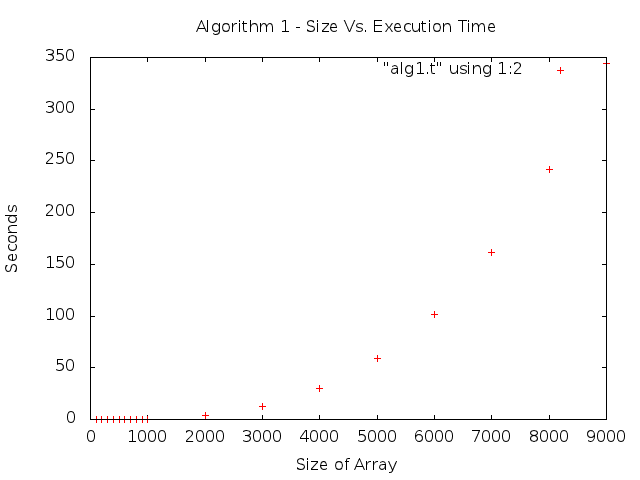
\includegraphics[scale=.5]{timingfiles/alg1plot.png}
			\end{figure}
			\begin{figure}[!htb]
				\centering
				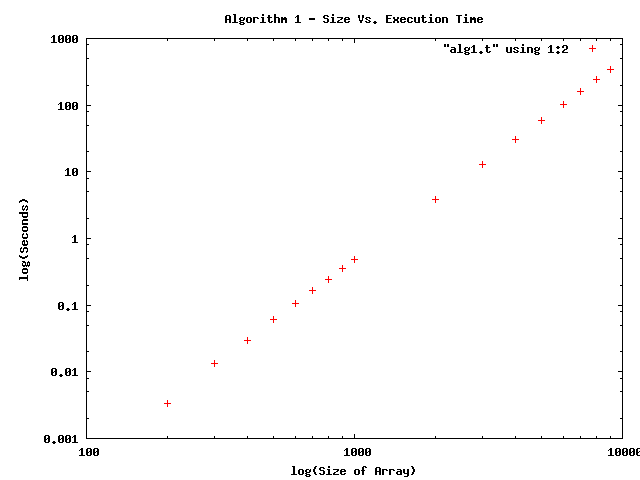
\includegraphics[scale=.5]{timingfiles/alg1plotlog.png}
			\end{figure}

		\newpage
		\subsection{Algorithm 2}
			\begin{figure}[!htb]
			\centering
			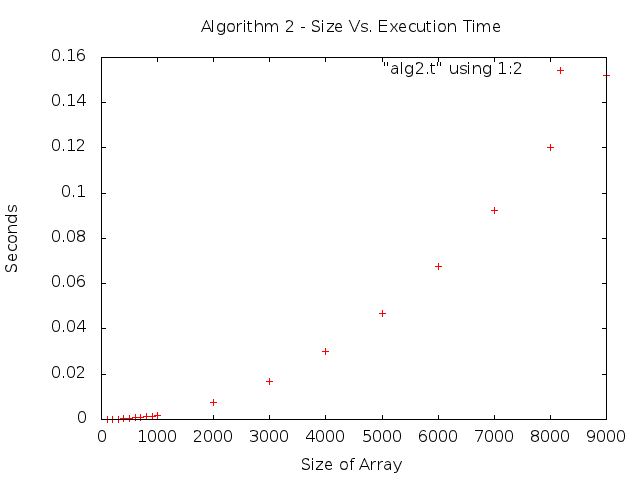
\includegraphics[scale=.5]{timingfiles/alg2plot.png}
			\end{figure}
			\begin{figure}[!htb]
			\centering
			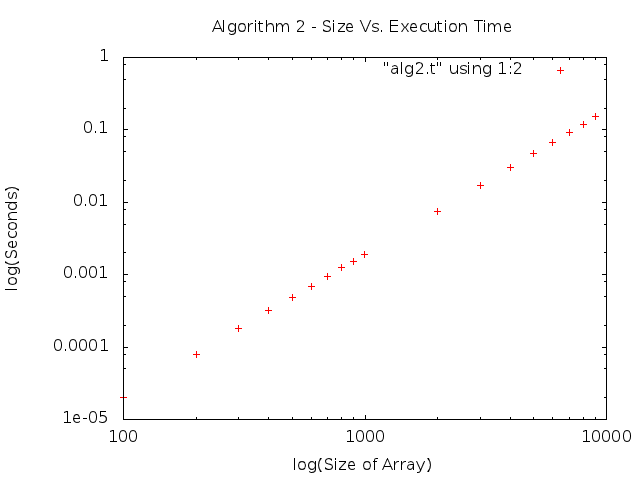
\includegraphics[scale=.5]{timingfiles/alg2plotlog.png}
			\end{figure}

		\newpage
		\subsection{Algorithm 3}
			\begin{figure}[!htb]
			\centering
			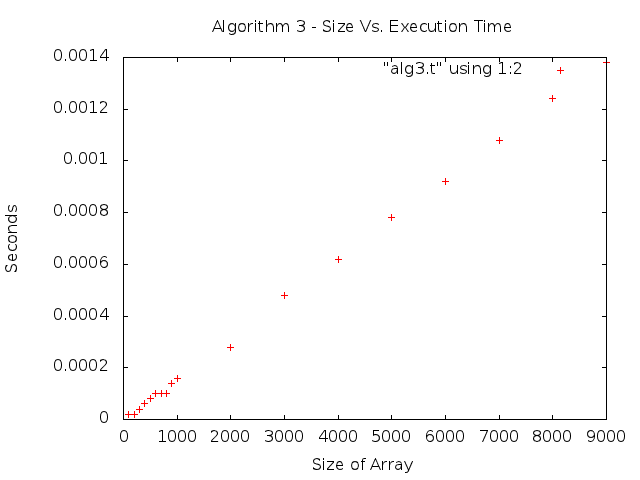
\includegraphics[scale=.5]{timingfiles/alg3plot.png}
			\end{figure}
			\begin{figure}[!htb]
			\centering
			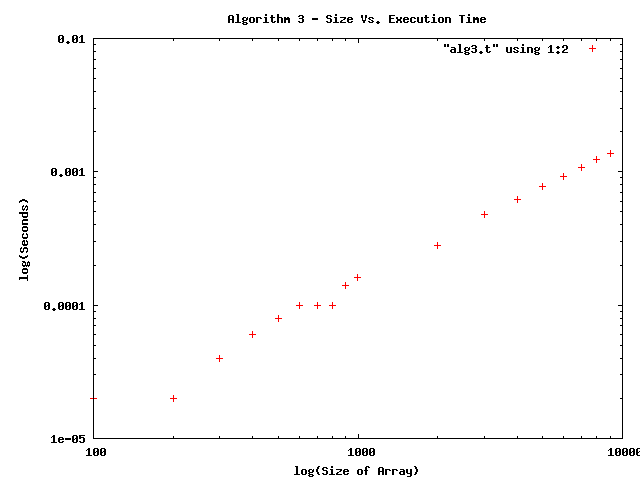
\includegraphics[scale=.5]{timingfiles/alg3plotlog.png}
			\end{figure}

	\newpage
	\section{Extrapolation and Interpretation}

		\subsection{Extrapolation}
			The functions were calculated using gnuplot's fit function.

		\subsection{Interpretation}
			The functions were calculated using gnuplot's fit function and fitting the data to $f(n) = 10^{m \log_{10}n+c}$
			The slopes for each algorithm is a little lower than the actual power because of the creation overhead of the function has a larger affect on arrays with small sizes.  This will cause the left side to be higher and therefore decreases slope.

		\subsection{Algorithm 1}
			\subsubsection{Extrapolation}
				$f(n) = 4.71599 \times 10^{-10} \times n^3$\\
				$f(n) = 3600 \to n = \boxed{19690}$
			\subsubsection{Interpretation}
				Slope $= \boxed{2.99734}$
		
		\subsection{Algorithm 2}
			\subsubsection{Extrapolation}
				$f(n) = 1.87761 \times 10^{-9} \times n^2$\\
				$f(n) = 3600 \to n = \boxed{1384678}$
			\subsubsection{Interpretation}
				Slope $= \boxed{1.99602}$

		\subsection{Algorithm 3}
			\subsubsection{Extrapolation}
				$f(n) = 1.74832 \times 10^{-8} \times n \times log(n)$\\
				$f(n) = 3600 \to n = 8984428998 = \boxed{8.98 \times 10^9}$
			\subsubsection{Interpretation}
				Slope $= \boxed{1.00506}$

	\newpage
	\section{Code}
		\subsection{Files}
			alg1.cpp - Function for algorithm 1\\
			alg2.cpp - Function for algorithm 1\\
			alg3.cpp - Function for algorithm 1\\
			analysis.cpp - Code to run algorithm and measure times for the number of array then outputs .t file\\
			makefile - To compile files\\
			maxSubarray.pdf - This writeup\\
			maxSubarray.tex - \TeX file for PDF\\
			test.cpp - Allows input of file and runs algorithm on input file\\
			analysis/ - Contains compiled executables for running analysis\\
			test/ - Contains compiled executables for running tests on code, and test array files\\
			timingfiles/ - Contains files for creating plots\\
			timingfiles/*.t - Log of runtimes for different array sizes\\
			timingfiles/*.gp - Code for gnuplot. 2 plots of each algorithm: 1 normal plot, and 1 log-log plot

		\subsection{Algorithm 1}
		\lstinputlisting[language=C++]{alg1.cpp}
		\newpage
		\subsection{Algorithm 2}
		\lstinputlisting[language=C++]{alg2.cpp}
		\newpage
		\subsection{Algorithm 3}
		\lstinputlisting[language=C++]{alg3.cpp}
		

\end{document}
